\tunemarkup{coverimage}{%
\newcommand{\adjustimg}{\checkoddpage\ifoddpage\hspace*{\dimexpr\evensidemargin-\oddsidemargin}\else\hspace*{-\dimexpr\evensidemargin-\oddsidemargin}\fi}
\newcommand{\centerimg}[2][width=\textwidth]{\makebox[\textwidth]{\adjustimg\includegraphics[#1]{#2}}}
\newpagecolor{ubpagecolor}\afterpage{\restorepagecolor}
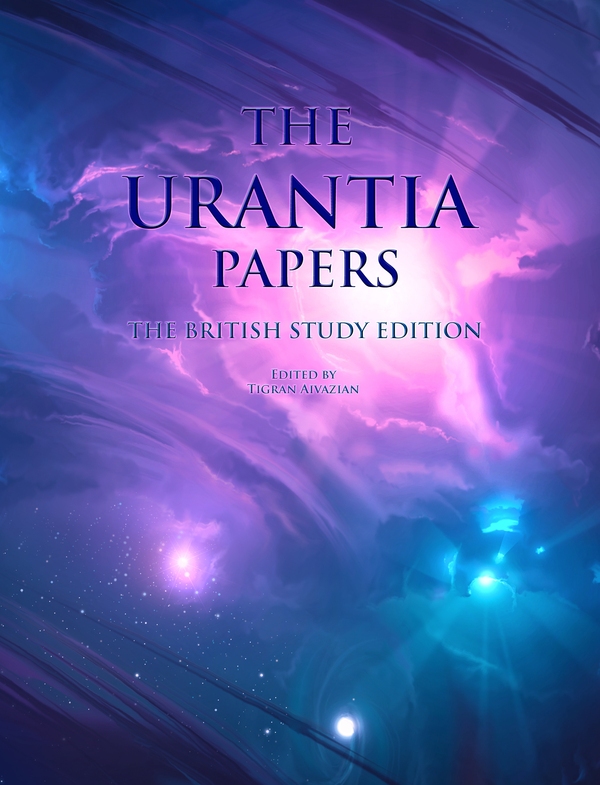
\includepdf{images/British-Study-Edition-Cover-tiny.png}
}

\makeatletter
\bib@raise@anchor{\bibpdfbookmark[0]{Title Page}{Ttl}}%
\makeatother

\vspace*{\stretch{0.1}}
\begin{center}
{
\booktitlefontsize THE BRITISH \tunemarkuptwo{nofnt}{TEXT}{STUDY} EDITION\\
\offontsize OF\\
\booksubtitlefontsize THE URANTIA PAPERS\\
}%
{%
\vspace*{\stretch{0.1}}
\tunemarkup{pghanlin}{\fontsize{10}{13}\selectfont}
\tunemarkup{pgkindledx}{\fontsize{16}{18}\selectfont}
\tunemarkup{pgcrownq}{\fontsize{19}{24}\selectfont}
\tunemarkup{pgafour}{\fontsize{21}{28}\selectfont}
\tunemarkup{pgnexus7}{\fontsize{10}{12}\selectfont}
\tunemarkup{pgthinmob}{\fontsize{10}{12}\selectfont}
\tunemarkup{pgnexus10}{\fontsize{15}{22}\selectfont}
\tunemarkup{pgkoboaurahd}{\fontsize{13}{17}\selectfont}
\tunemarkup{pgauraone}{\fontsize{13}{15}\selectfont}
\itshape
The Revised Text in British English\tunemarkuptwo{nofnt}{\\[2ex]}{%
,\\
With \totalnfnsts\ Notes \&\ \totalfigures\ Illustrations\\[2ex]
}
Edited by Tigran Aivazian\\[2ex]
\tunemarkuptwo{noquiz}{}{With Interactive Cosmic Citizenship Quiz\\Of \totalcurqs\ Questions\\}
}%
\ifmultivol
\LARGE\bfseries\itshape
\ifvoli Volume I: Foreword \&\ Papers 1--96\\\fi
\ifvolii Volume II: Papers 97--196\\\fi
%\ifvoliii Volume III: Papers 129--196\\\fi
\fi
\vspace*{\stretch{0.4}}

\includegraphics[width=0.2\columnwidth]{images/Phoenix-Logo-Circles.jpg}\\
\vspace*{\stretch{0.3}}
\titlesepbig\\
\vspace*{\stretch{0.1}}
\end{center}

\titleframe

\newpage

%\newcommand{\serpimolot}{{\fontspec{Mortbats} K}}

\begin{center}
\vspace*{\stretch{0.3}}
\begin{center}\shadowbox{\strut\parbox{7cm}{\normalsize\tunemarkup{pgnexus10}{\large}\tunemarkup{pgkindledx}{\Large}\tunemarkup{pgcrownq}{\Large}\tunemarkup{pgafour}{\large}\bfseries\itshape ``One of the most important things in human living is to find out what Jesus believed, to discover his ideals, and to strive for the achievement of his exalted life purpose.'' \bibref[(196:1.3)]{p196 1:3}}}\end{center}
\vspace*{\stretch{0.5}}
\infofontsize
\parbox{0.9\linewidth}{\centering
\textbf{\upshape\nocopyright\ No copyright is claimed on this book\\
The text of \bibemph{The Urantia Papers} is in the public domain.}\\[5pt]
\tunemarkuptwo{coverimage}{Cover design by Gary Tonge.\\}{}
The latest version of this book can be downloaded from:\\
{\upshape\bfseries http://www.bibles.org.uk}\\
Please send all comments to: {\makeatletter\upshape\bfseries aivazian.tigran@gmail.com\makeatother}\\[1ex]
\tux\ Typeset with \XeLaTeX\ of \TeX\ Live 2020 under Linux.\\
English text set in {\bfseries\tunemarkup{garamond}{Adobe }\urantiamainfont\tunemarkup{garamond}{ Opticals}} at \urantiamainfontsize pt.\\
Hebrew text set in {\bfseries\hebrewfontname.}\\
Greek text set in {\bfseries\greekfontname.}\\
Armenian text set in {\bfseries Tarumian GrqiBardzr.}\\
Chinese text set in {\bfseries\chinesefontname.}\\[10pt]
\upshape\tunemarkup{pgcrownq}{\large}\tunemarkup{pgafour}{\Large}\bfseries PDF version: \tunemarkup{pgthinmob}{20:9 Colour}\tunemarkup{pgcrownq}{Crown Quarto}\tunemarkup{pgafour}{A4}\tunemarkup{pgnexus7}{7" Colour}\tunemarkup{pgnexus10}{10" Colour}\tunemarkup{pghanlin}{6" eInk}\tunemarkup{pgkobomini}{5" eInk}\tunemarkup{pgkoboaurahd}{7" eInk}\tunemarkup{pgkindledx}{10" eInk}\tunemarkup{pgauraone}{8" eInk}\\
\upshape\bfseries PDF date: \mytoday{}\\
}
\vspace*{\stretch{0.1}}
\end{center}

\titleframe
